Communication as mentioned before is a key part of AVs.
A Vehicular ad hoc network (VANET) is a proposed type of mobile ad hoc network (MANET) involving road vehicles.
This type of network permits vehicles to communicate with roadside equipment, such as traffic lights, and with each other\cite{sheikh2019comprehensive}.
For example, VANETs can be used for vehicle-to-vehicle (V2V) and Vehicle-to-Infrastructure (V2I) communications, so for external communications.
The main purpose of such technology is to generate security on the roads, in this case security in terms of passengers and pedestrian safety.
The main components of VANET technology are: \textit{On-board unit (OBU)}, \textit{Road-side unit (RSU)}, \textit{Trusted Authority (TA)}.
The Trusted Authority acts as a key part in the VANET architecture,
as it is responsible for managing the security of the network and ensuring that all vehicles are authenticated
and authorized to communicate.

Communications are crucial for Autonomous Vehicles (AVs) to interact with other vehicles, infrastructure, and the cloud.
There are various ways to categorize communication in AVs. One approach is based on the range of communication, while another can be based on the type of communication, depending on the focus.
For example, communication in AVs can be classified either by range:
\begin{enumerate}
    \item \textbf{Short-range communication}
    \item \textbf{Medium-range communication}
    \item \textbf{Long-range communication}
\end{enumerate}

Or by the type of interaction:
\begin{enumerate}
    \item \textbf{Vehicle-to-Vehicle (V2V)}
    \item \textbf{Vehicle-to-Infrastructure (V2I)}
    \item \textbf{Vehicle-to-Everything (V2X)}
\end{enumerate}

To favor the type of communications instead of the range, the following sections will be based on the type of interaction.

\subsection{Vehicle-to-Vehicle (V2V)}\label{subsec:vehicle-to-vehicle-(v2v)}

The V2V communication provides several advantages that can be exploited, such as the Blind Spot Detection (BSD) that warns the drivers about other vehicles of any type located out of sight,
the Forward Collision Warning System (FCWS), automatic emergency braking (AEB) and the Lane departure warning system (LDWS)\cite{arena2019overview}.

Vehicle-to-Vehicle (V2V) technology involves wireless communication between motor vehicles, aiming primarily to prevent accidents by exchanging data such as position and speed.
This communication happens within an ad-hoc mesh network, which can either be fully connected or partially connected.
In both cases, messages can be relayed directly or through multiple paths, ensuring robust communication even if some nodes fail.
While wired mesh networks were once expensive and challenging to implement, wireless technologies, such as WPANs, have made them more feasible today\cite{arena2019overview}.

Depending upon the number of hops used for inter-vehicle communication, they are classified as single-hop (SIVC) or
Multi-hop (MIVC) systems.
The SIVC can be used for short-range applications such as
lane merging, adaptive cruise control, etc., whereas MIVC can be used for long-range communication such as traffic monitoring\cite{zheng2020cooperative}.

The USDOT (Department of Transportation of the United States of America) has documented the security requirements of
systems and in particular, the need to define security network requirements for V2V and its supporting systems.

\subsection{Vehicle to Infrastructure (V2I)}\label{subsec:vehicle-to-infrastructure-(v2i)}
Vehicle to Infrastructure is another type of communication as a key part of the intelligent transportation system (ITS)
that enables vehicles to communicate with roadside infrastructure, such as traffic lights, signs, and road sensors.
It represents the next evolution in Intelligent Transportation Systems (ITS)~\cite{dot2024v2i}.

State and local agencies are expected to install V2I systems either alongside or integrated with existing ITS equipment.
As a result, many V2I deployments could be eligible for similar federal-aid programs as ITS,
provided the deploying agency meets certain requirements\cite{dot2024v2i}.

\subsection{Vehicle to Everything (V2X)}\label{subsec:vehicle-to-everything-(v2x)}

Vehicle-to-Everything (V2X) is a general communication model that generalizes Vehicle-to-Vehicle (V2V) and Vehicle-to-Infrastructure (V2I) systems,
incorporating interactions between vehicles and other entities, such as pedestrians (V2P)~\cite{vehicle-to-pedestrian}, roadside equipment (V2R)~\cite{vehicle-to-roadside}, and devices (V2D).
V2X, like V2V and V2I, aims to enhance road safety, focussing on vulnerable road users.

\begin{figure}[!htb]
    \centering
    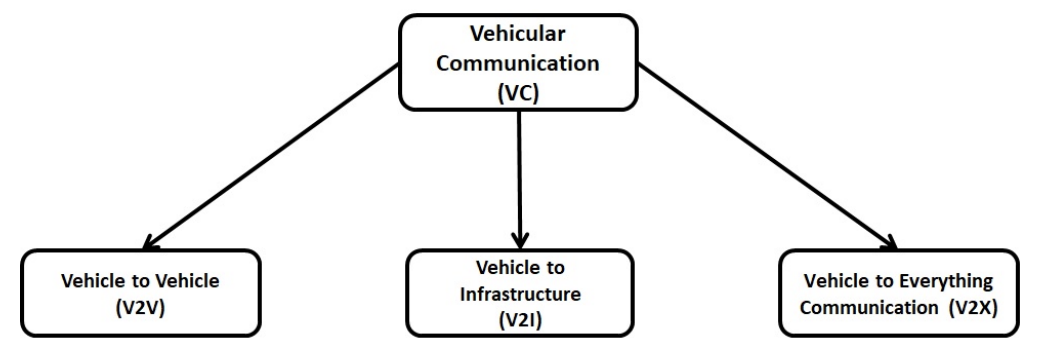
\includegraphics[width=0.7\linewidth]{figures/communication}
    \caption{VANETs}
    \label{fig:communication}
\end{figure}

\subsection{Can BUS Communication}\label{subsec:canbus-communication}
Internal communications are managed by the Controller Area Network (CAN) bus.
CAN is the most common network topology used for controlling the automotive and the industrial system.
It is a communication network that offers rapid communication among microcontroller
devices.
CAN employ interconnected nodes to send a message-based protocol designed to
permit all nodes to receive the message and perform on the network message\cite{canbus}.
CAN is the standard bus interface that attackers use to inject attack messages into the
communication network, it requires to be located near the target vehicle to perform the attack if the exploitation is only physical and not through the network; in that case, the attacker can be located anywhere in the world.
The CAN bus is a broadcast network, meaning that all nodes on the network receive the message and require no authentication to receive the message, that is hazardous in terms of security.
Researchers tried to evaluate some new technologies to detect the malicious code and mitigate the attacks\cite{aldhyani2022attacks}\ref{subsec:artificial-intelligence} using deep learning algorithms to detect the malicious code on the CAN bus.
The proposed systems have demonstrated effective detection of abnormal packets to safeguard the CAN bus.
Additionally, they can be adapted to other security system designs within the complex infrastructures of autonomous vehicle networks, ensuring more secure data processing.
